\newpage
\section{Durchführung}
\label{sec:durchfuehrung}

Der Aufbau und die Durchführung variieren für die einzelnen Schaltungen, da mehrere Effekte untersucht werden sollen.
Alle Schaltungen sind auf dem Operationsverstärker LM741 basiert\cite{lm741}.
In \autoref{fig:ov} sind dessen innerer Aufbau, sowie die verschiedenen Außenkontakte dargestellt.

\begin{figure}[H]
    \centering
    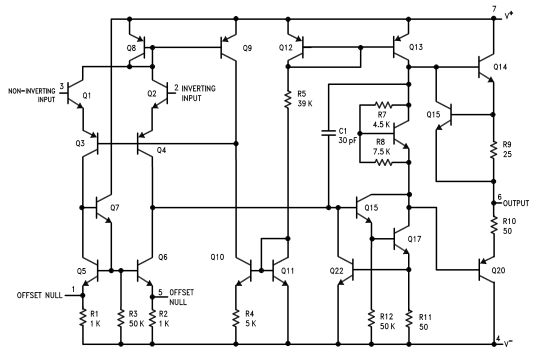
\includegraphics[scale=0.7]{images/innerer_aufbau.png}
    \caption{Innerer Aufbau des Operationsverstärkers LM741.\cite{lm741}}
    \label{fig:ov}
\end{figure}

Als Versorgungsspannung werden $\pm$\SI{15}{\volt} angeschlossen.
Die Eingangsspannung wird von einem Funktionsgenerator gespeist.
Sowohl die Eingangsspannung als auch die Ausgangsspannung werden auf einem Oszilloskop graphisch dargestellt.

\subsection{Invertierender Linearverstärker}
Die in \autoref{fig:linear2} dargestellte Schaltung auf einem Breadboard so aufgebaut, dass die Widerstände modular sind und Ein- und Ausgangssignal auf dem Oszilloskop sichtbar sind.

\begin{figure}[H]
    \centering
    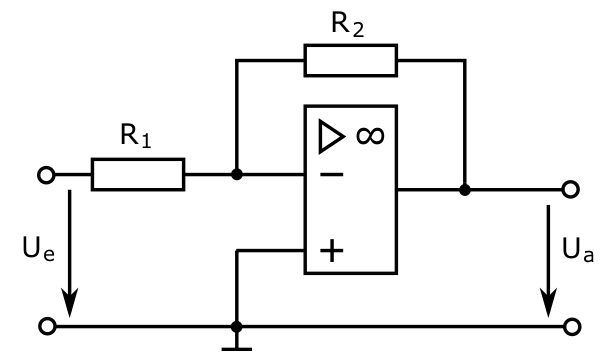
\includegraphics[scale=0.5]{images/linear.png}
    \caption{Aufbau eines invertierenden linearen Verstärkers.\cite{V51}}
    \label{fig:linear2}
\end{figure}

Mit insgesamt drei verschiedenen Widerstands-Paaren wurden mehrere Frequenzbereiche des \SI{140}{\milli\volt} peak-to-peak Eingangssignals angelegt.
Die Messung der Phasenverschiebung, sowie der Abfall der Verstärkung wird mit der Analyse Funktion des Oszilloskops gemessen.
Die gesammelten Daten sollen für alle drei Verstärkungsfaktoren doppelt logarithmisch aufgetragen und durch die Abfallkurve ein Fit gelegt werden.
Die Phase wird separat geplottet.

\subsection{Umkehr-Integrierer}
Der Aufbau des Umkehr-Integrierers ist in \autoref{fig:integr} dargestellt.

\begin{figure}[H]
    \centering
    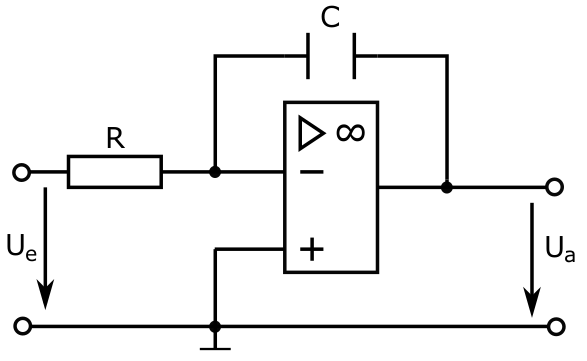
\includegraphics[scale=0.5]{images/integrierer.png}
    \caption{Aufbau eines Umkehr-Integrierers.\cite{V51}}
    \label{fig:integr}
\end{figure}

Die verbauten Komponenten sind ein \SI{10}{\kilo\ohm} Widerstand und ein \SI{100}{\nano\farad} Kondensator.
Bei steigender Frequenz des Eingangssignals wurden die Eingangsspannung und Ausgangsspannung gemessen.
Ein doppelt logarithmisches Diagramm von Frequenzwerten zu Ausgangsspannungsmesswerten sollte geplottet werden.
Die in \autoref{eq:integrierer} beschriebene Relation soll anhand der Spannungen dargestellt werden.\\
Für jeweils eine sinusförmige, dreiecksförmige und eine Rechteckfrequenz sollen die Messlinien des Oszilloskops abgebildet werden.

\subsection{Invertierender Differenzierer}
Der Aufbau des invertierenden Differenzierers ist in \autoref{fig:diff} dargestellt.

\begin{figure}[H]
    \centering
    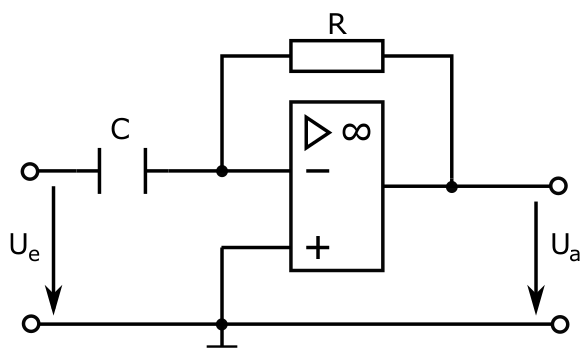
\includegraphics[scale=0.5]{images/differenzierer.png}
    \caption{Aufbau eines invertierenden Differenzierers.\cite{V51}}
    \label{fig:diff}
\end{figure}

Die verbauten Komponenten sind ein \SI{22}{\nano\farad} Kondensator und ein \SI{100}{\kilo\ohm} Widerstand.
Es soll das gleiche gemessen werden, wie beim Umkehr-Integrierer.

\subsection{Nicht-Invertierender Schmitt-Trigger}
Die Schaltung des nicht-invertierenden Schmitt-Triggers ist in \autoref{fig:schmitt} dargestellt.

\begin{figure}[H]
    \centering
    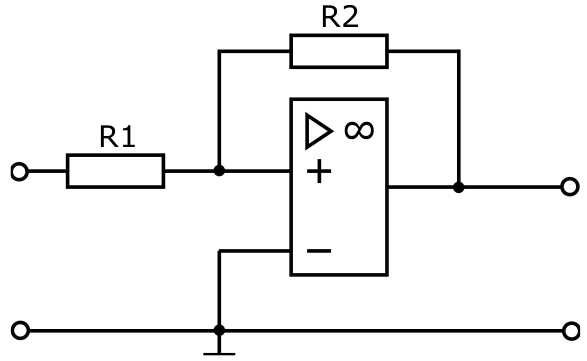
\includegraphics[scale=0.5]{images/trigger.png}
    \caption{Aufbau eines nicht-invertierenden Schmitt-Triggers.\cite{V51}}
    \label{fig:schmitt}
\end{figure}

Die genutzten Bauteile sind zwei Widerstände mit den Werten $R_1 = $\SI{10}{\kilo\ohm} und $R_2 = $\SI{100}{\kilo\ohm}.
Die Eingangsspannung wurde in kleinen Schritten erhöht, bis die Schaltung kippt.
Dieser Scheitelwert soll mit dem theoretischen Wert verglichen werden und das entstandene Bild vom Oszilloskop mit Ein- und Ausgangsspannung dargestellt werden.

\subsection{Signalgenerator}
Für die Schaltung des Signalgenerators wird parallel hinter den Schmitt-Trigger ein Umkehr-Integrator geschaltet, wie in \autoref{fig:signal} zu sehen ist.

\begin{figure}[H]
    \centering
    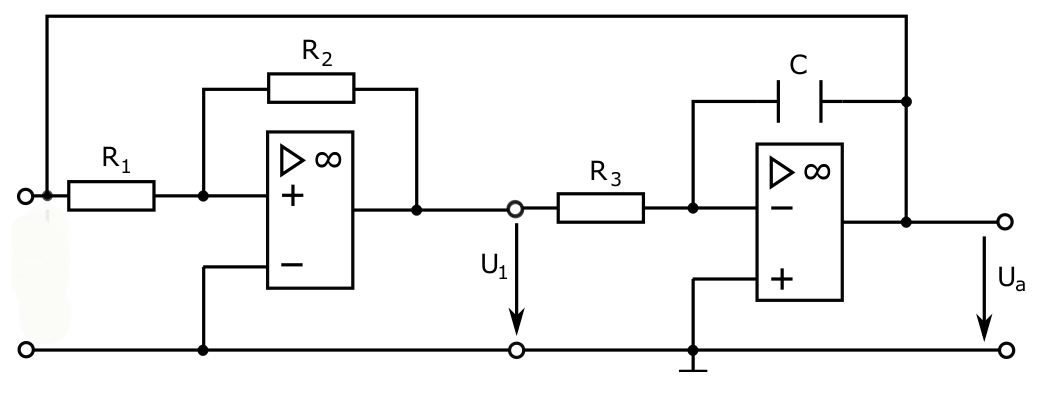
\includegraphics[width=\textwidth]{images/signal.png}
    \caption{Aufbau eines Signalgenerators.\cite{V51}}
    \label{fig:signal}
\end{figure}

Die Widerstände werden aus dem Schmitt-Trigger übernommen.
Der Widerstand $R_3$ und der Kondensator $C$ haben die Werte \SI{1}{\kilo\ohm} und \SI{1}{\micro\farad}.\\
Bei dieser Schaltung wird keine Eingangsspannung benötigt.
Stattdessen werden nur die Ausgangsspannung und die Spannung $U_1$ zwischen Schmitt-Trigger und Umkehr-Integrierer auf dem Oszilloskop betrachtet.
Wie in der \autoref{fig:signal} zu sehen ist, wird der Ausgang des Integrierers zurück auf den nicht-invertierenden Eingang des Schmitt-Triggers geleitet.
Die auf dem Oszilloskop zu sehende Dreieck-Schwingung soll mit den theoretischen Werten für Amplitude und Frequenz verglichen werden.